\documentclass[mathserif, 13pt, aspectratio=1610]{beamer}
\usetheme{Frankfurt}

\usepackage{subcaption}
\usepackage{graphicx} % for including figures
\usepackage{hyperref}
\setbeamertemplate{caption}[numbered]


\usepackage{tabularx}
\usepackage{booktabs} % For better table rules

% ++++++++++++++++++++++++++Code global config begin++++++++++++++++++++++++++
% Code block universal settings, all lstdefinestyle must appeared below this block!
\usepackage{listings}
% use txtt global font
\usepackage[T1]{fontenc} % Add font options
\DeclareFixedFont{\codefont}{T1}{txtt}{m}{n}{12} % other options: txtt -> cmtt, pcr, fvm, zi4; m -> bx, n; 12 -> (fontsize)

% Define colors
\usepackage{color}
\usepackage{tikz} % colorlet need this
\definecolor{commentgreen}{rgb}{0,0.5,0}
\colorlet{framegray}{black!40}
\definecolor{stringred}{rgb}{0.6,0,0}

% Global config
\lstset{
	backgroundcolor=\color{gray!7},
	% numbers = left, % show line number on the left
	% numberstyle = \small\color{framegray}, % line number color
	basicstyle = \codefont, % code font
	columns = flexible, % make the spacing between characters compact
	keepspaces = true,  % keeps spaces in text, useful for keeping indentation of code (needs columns=flexible)
	% captionpos = b, % caption at the bottom
	commentstyle = \color{commentgreen}, % comment color
	frame = single, % display frame
	stringstyle = \color{stringred}, % Strings in red
	rulecolor = \color{framegray}, % frame color
	showstringspaces = false, % don't mark spaces in strings
	breaklines = true, % break long lines
	tabsize = 4, % tab size
}
% +++++++++++++++++++++++++++Code global config end+++++++++++++++++++++++++++

% ++++++++++++++++++++++++++Bash local config begin++++++++++++++++++++++++++
% Must placed below the global settings
% this will override the global settings
\lstdefinestyle{custombash}{
	language = bash,
	basicstyle = \ttfamily, % Monospaced font
	keywordstyle = \color{blue}\bfseries, % Keywords in bold blue
	stringstyle = \color{green}, % Strings in green
	commentstyle = \color{gray}, % Comments in gray
	morekeywords = {sudo, ls, cd, rm, mkdir}, % Add common Bash commands
}
% +++++++++++++++++++++++++++Bash local config end+++++++++++++++++++++++++++


\setbeamertemplate{navigation symbols}{} % Do not show navigation symbols
\setbeamercovered{transparent} % Show covered items in a transparent way

\title{Source Coding for \textit{the Game of Thrones}}
\subtitle{2nd-Order Markov Adaptive Approximation (AME), Huffman, and Fano Coding}
\author[Jinming Ren (2022190908020), Yuhao Liu (2022190908022)]{Jinming Ren (2022190908020, Presenter) \\ Yuhao Liu (2022190908022) \\
        \vspace{1em} % Add some spacing
        \tiny{\textbf{University of Glasgow}} \\
        \vspace{0.3em}
        \tiny{\textbf{University of Electronic Science and Technology of China}} \\
}
\date{\today}

\begin{document}

\begin{frame}
  \titlepage
\end{frame}

\begin{frame}{Overview}
  \tableofcontents
\end{frame}


\section{Motivation and Main Research Findings}
\begin{frame}{Background}
	\begin{columns}[T]
		\column{0.5\textwidth}
		\centering
		\hfill
		\begin{itemize}
			\item \textbf{Goal:} Compress text (first 3 chapters of \textit{the Game of Thrones}) effectively using a source coding method.
		\end{itemize}

		\begin{theorem}[Source Coding Theorem]
			$$
			\bar{L} \geq H(X)
			$$
		\end{theorem}

		\begin{itemize}
			\item \textbf{Entropy Coding:} What's beyond?
			\begin{itemize}
				\item Huffman
				\item Fano
				\item Arithmic
				\item $\cdots$
			\end{itemize}
			\item ``Memoryless Assumption''
		\end{itemize}

		\lstinputlisting[language=bash, style=custombash]{example-sentence.txt} % bash


		\column{0.4\textwidth}
		\centering
		\begin{figure}[h!]
			\centering
			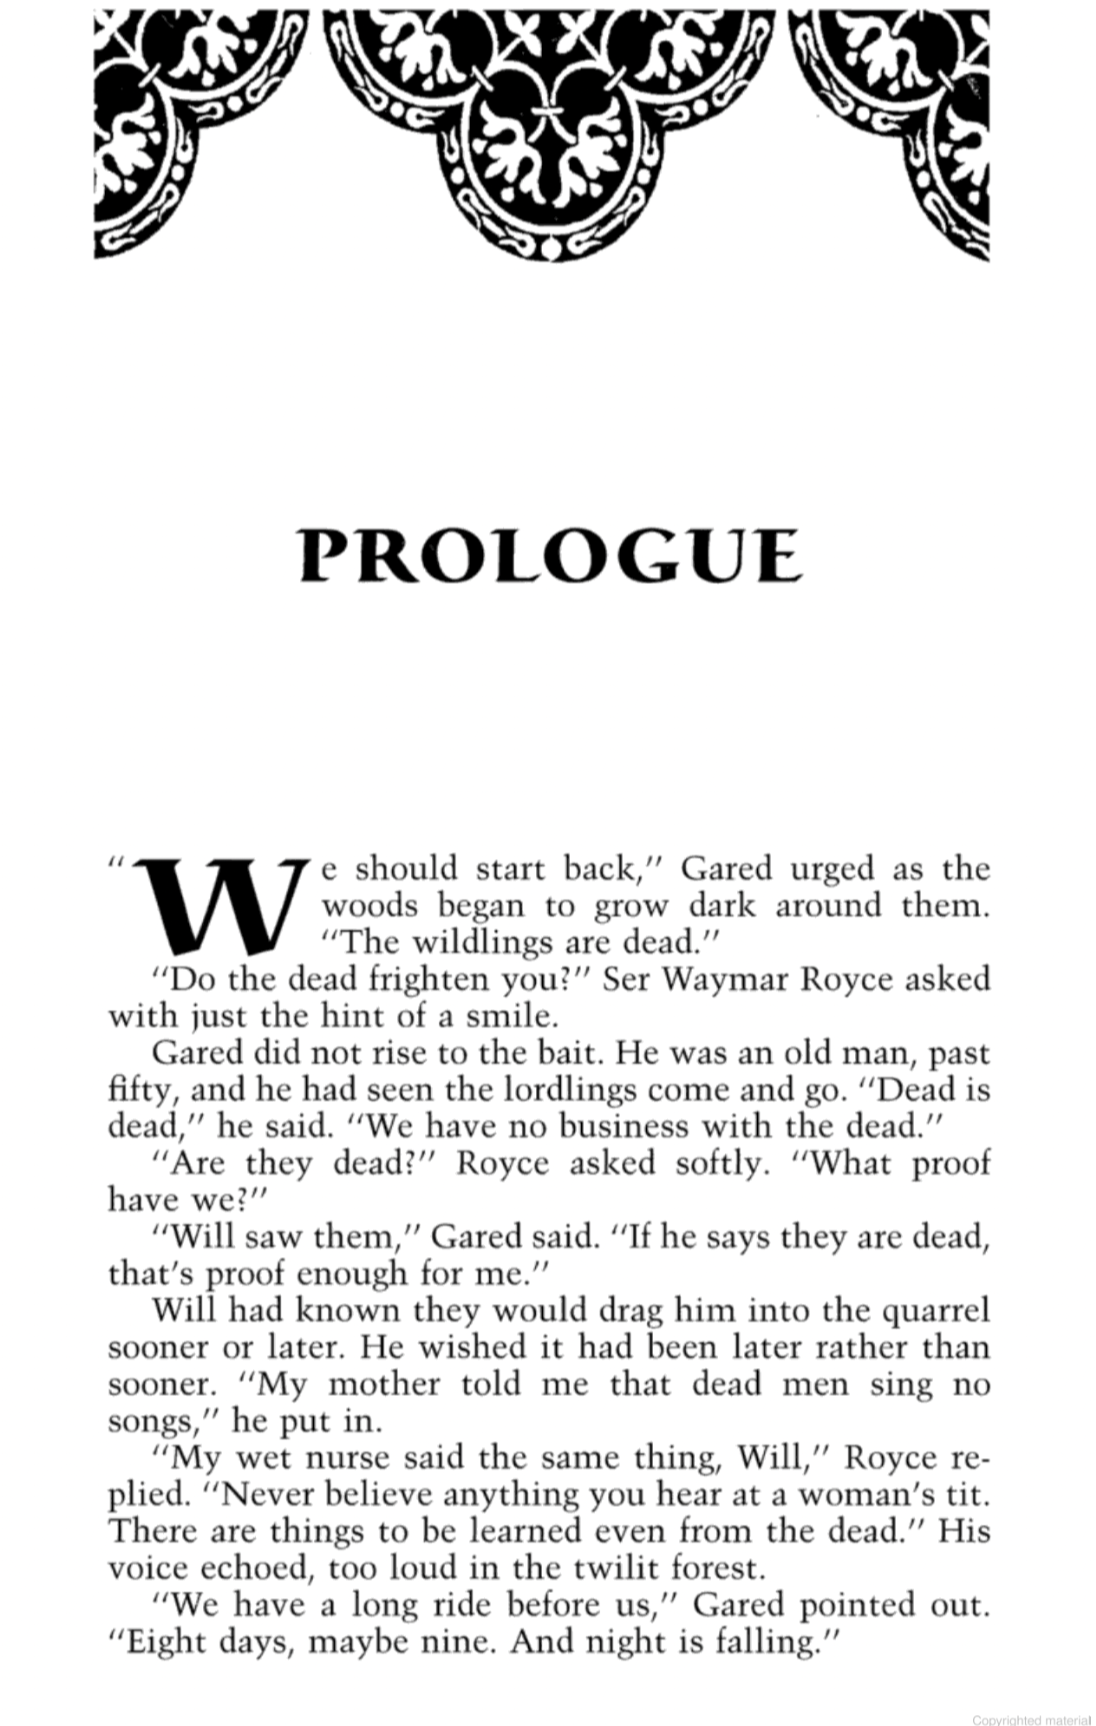
\includegraphics[width=0.75\textwidth]{the-game-of-thrones.png}
			\caption{\textit{The Game of Thrones} by George R. R. Martin}
			\label{fig:the-game-of-thrones}
		\end{figure}
	\end{columns}
\end{frame}


\begin{frame}{Motivation}
	\begin{columns}[T]
		\column{0.5\textwidth}
		\centering
		\begin{itemize}
			\item \textbf{Non-entropy Coding:} Respect the internal structure of the source.
			\begin{itemize}
				\item LZ family (LZ77, LZ78, LZW, LZMA, LZSS)
				\item PPM (Prediction by Partial Matching)
				\item DMC (Dynamic Markov Compression)
				\item ML-based
				\item $\cdots$
			\end{itemize}
			\item Common point: ``Prediction''!
		\end{itemize}
		\column{0.5\textwidth}
		\centering
		\begin{figure}[h!]
			\centering
			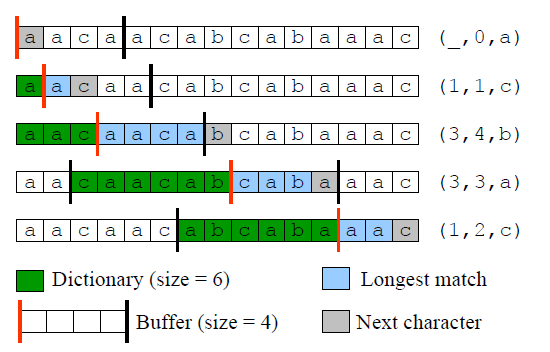
\includegraphics[width=1.05\textwidth]{lz77.png}
			\caption{LZ77 Compression}
			\label{fig:lz77}
		\end{figure}
	\end{columns}
	
\end{frame}


\begin{frame}{The Future of Lossless Source Coding}
	\textbf{Compression = Prediction}
	\begin{figure}[h!]
		\centering
		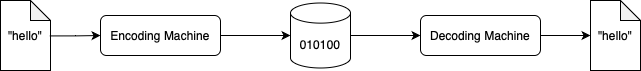
\includegraphics[width=\textwidth]{encode-decode-machine.png}
		\caption{Same deterministic machines at the sender and the receiver}
		\label{fig:encode-decode-machine}
	\end{figure}
	\begin{block}{Claim 1}
		A good compressor is also a good predictor.
	\end{block}
	\begin{block}{Claim 2}
		The bit stream from a good compressor should be unpredictable.
	\end{block}

\end{frame}


\section{AME Implementation Scheme}
\begin{frame}{Implementation Flowcharts}
	\begin{columns}[T]
	\column{0.45\textwidth}
		\begin{figure}[h!]
		\centering
		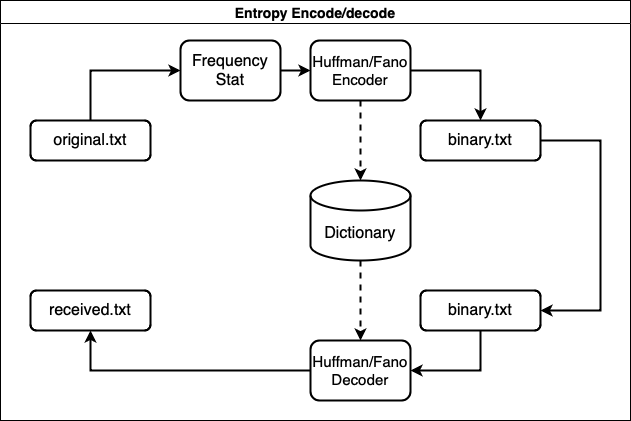
\includegraphics[width=\textwidth]{without-ame.png}
		\caption{Without AME}
		\end{figure}
	\column{0.61\textwidth}
		\begin{figure}[h!]
		\centering
		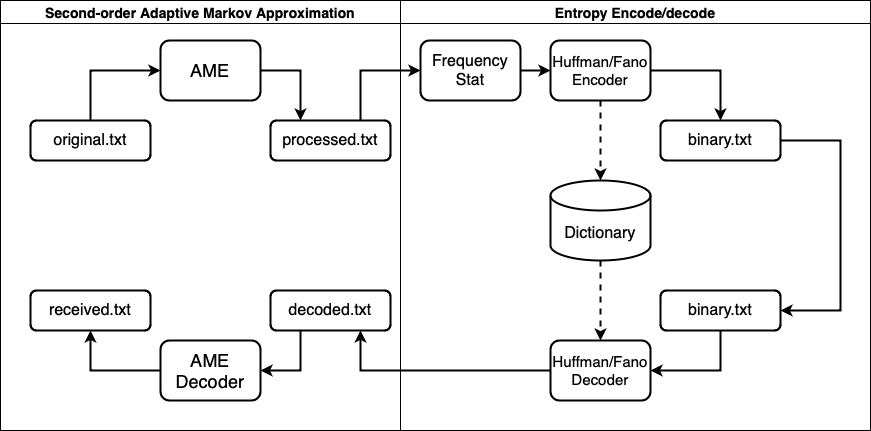
\includegraphics[width=\textwidth]{with-ame2.png}
		\caption{With AME}
		\end{figure}
	\end{columns}
\end{frame}


\begin{frame}{Inside AME Block}
	\begin{columns}[T]
		\column{0.5\textwidth}
		\centering
		\lstinputlisting[language=bash, style=custombash]{example-text-input.txt} % bash
		\column{0.5\textwidth}
		\centering
		\lstinputlisting[language=bash, style=custombash]{example-text-output.txt} % bash
	\end{columns}
	\begin{figure}[h!]
		\centering
		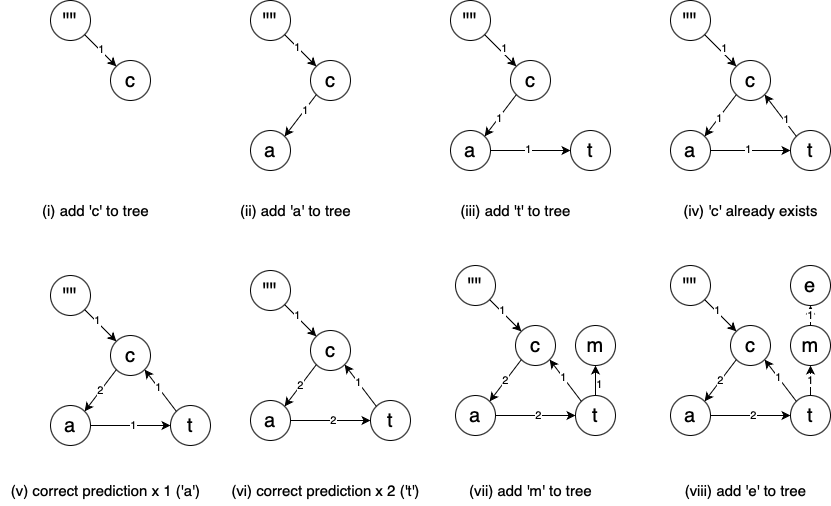
\includegraphics[width=0.75\textwidth]{AMEtree.png}
		\caption{Example: Contruction of an AME tree}
	\end{figure}
\end{frame}

\begin{frame}{AME Processed Text}
	\lstinputlisting[language=bash, style=custombash]{original_partof.txt} % bash
	\vfill
	\lstinputlisting[language=bash, style=custombash]{processed_part.txt} % bash
\end{frame}

\begin{frame}{Frequency Statistics Comparison}
	\begin{figure}[h!]
		\centering
		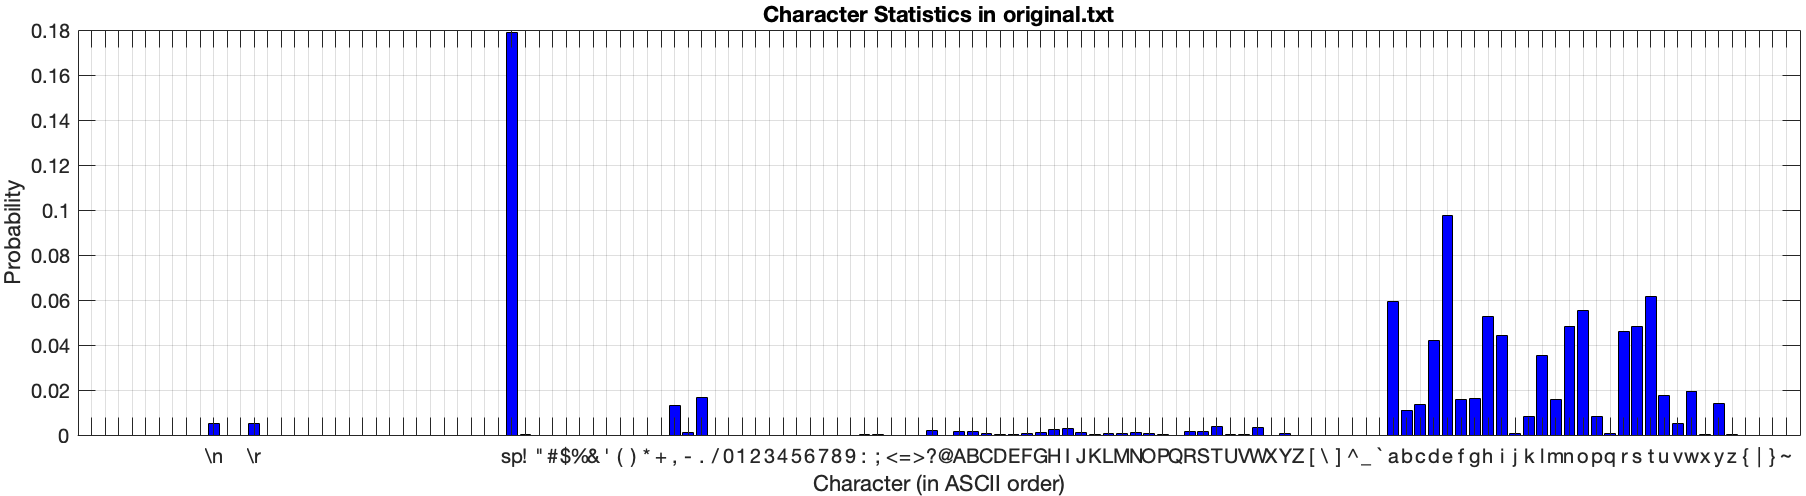
\includegraphics[width=0.9\textwidth]{originalStat.png}
	\end{figure}
	\begin{figure}[h!]
		\centering
		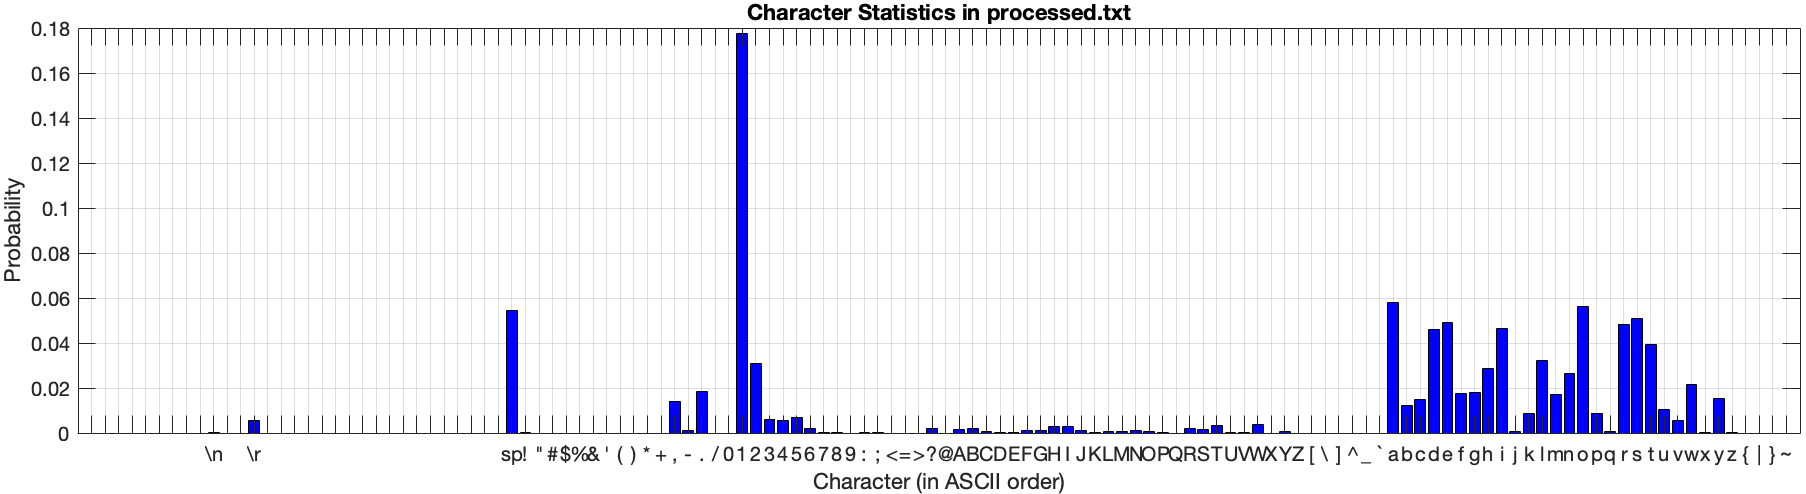
\includegraphics[width=0.9\textwidth]{processedStat.png}
	\end{figure}
\end{frame}


\section{Performance Analysis}
\begin{frame}{Compression Performance}
	\begin{columns}[T]
	\column{0.53\textwidth}
		\centering
		\begin{figure}[h!]
			\centering
			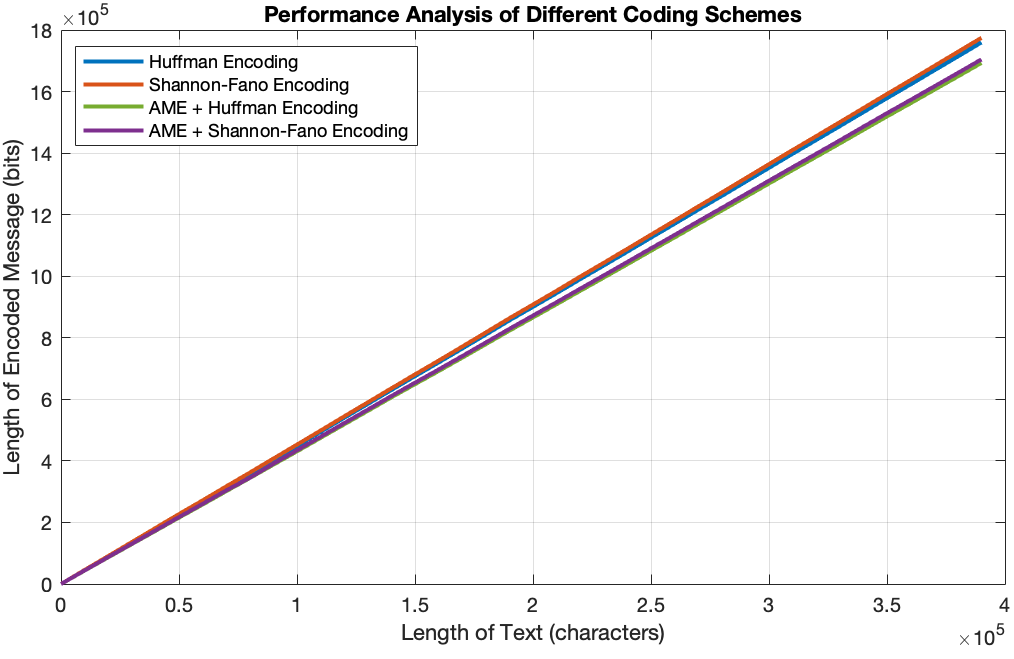
\includegraphics[width=\textwidth]{performanceAME1.png}
			\caption{Performance Comparison}
		\end{figure}
	\column{0.55\textwidth}
		\centering
		\begin{figure}[h!]
			\centering
			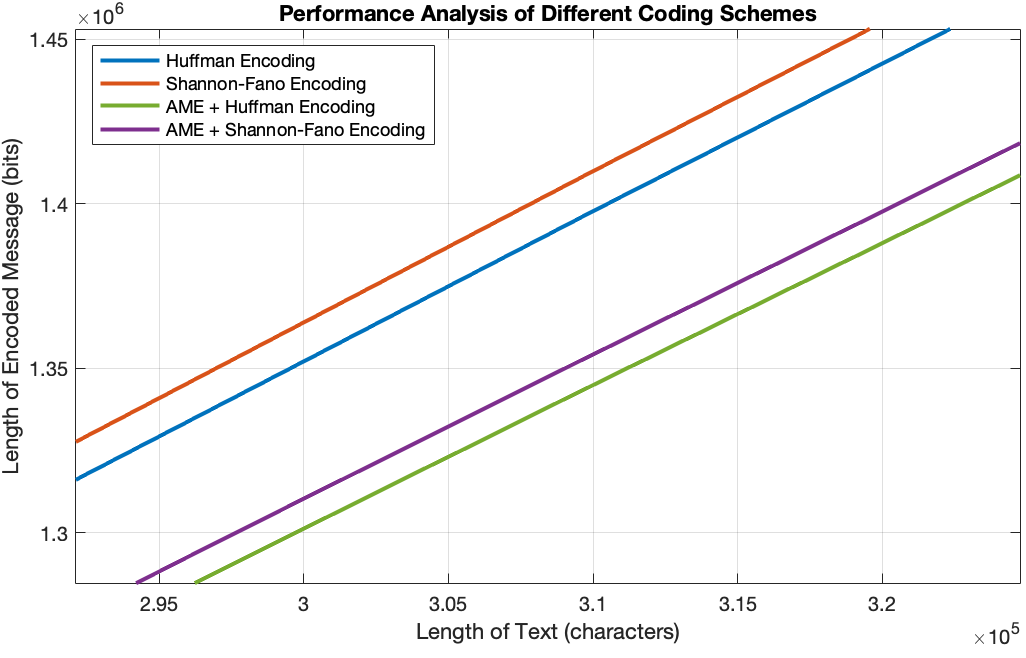
\includegraphics[width=\textwidth]{performanceAME2.png}
			\caption{Zoomed-in View}
		\end{figure}
	\end{columns}
\end{frame}

\begin{frame}{Compression Performance (Cont'd)}
	\begin{table}[h!]
		\small
		\caption{AME shortened the length of the binary file}
		\label{tab:amematrics}
		\centering
		\begin{tabular}{l|cccc}
		\toprule
		\textbf{Method} & \textbf{$\bar{L}$} & \textbf{With AME} & \textbf{Without AME} & \textbf{Improved} \\ \hline
		Huffman & 4.5 b/char & 207797 b & 217014 b & 5.25\%  \\ 
		Fano & 8.4 b/char & 209343 b & 218913 b & 4.37\% \\ 
		\bottomrule
		\end{tabular}
	\end{table}
\end{frame}


\section{Conclusion and Future Work}
\begin{frame}{Conclusion and Future Work}
	\begin{itemize}
		\item \textbf{Huffman vs. Fano:} Huffman is typically better.
		\item \textbf{AME's Advantage:} Pre-processing text to capture the ``memoryless'' component of the source.
		\item \textbf{Overall Gains:} A modest but consistent improvement of \(\approx4-5\%\) in code length for this text. 
		\item \textbf{Future Work:}
		\begin{itemize}
			\item Higher-order Markov models.
			\item Fast speed neural network models.
			\item Breakthrough in Linguistics, uncover general pattern in language syntax.
		\end{itemize}
	\end{itemize}
\end{frame}


\begin{frame}{References}
	\tiny
	\begin{thebibliography}{99}
		\bibitem{ref1} C. E. Shannon, ``A Mathematical Theory of Communication,'' \textit{The Bell System Technical Journal}, vol. 27, no. 3, pp. 379–423, July 1948, doi: 10.1002/j.1538-7305.1948.tb01338.x.

		\bibitem{ref6} J. Ziv and A. Lempel, “A universal algorithm for sequential data compression,” \textit{IEEE Trans}. Inform. Theory, vol. 23, no. 3, pp. 337–343, May 1977, doi: 10.1109/TIT.1977.1055714.
	
		\bibitem{ref7} A. D. Wyner and J. Ziv, “The sliding-window Lempel-Ziv algorithm is asymptotically optimal,” \textit{Proc. IEEE}, vol. 82, no. 6, pp. 872–877, Jun. 1994, doi: 10.1109/5.286191.
	
		\bibitem{ref5} T. Sharma et al., ``A Survey on Machine Learning Techniques for Source Code Analysis,'' Sep. 13, 2022, arXiv: arXiv:2110.09610. doi: 10.48550/arXiv.2110.09610.
	
		\bibitem{ref2} Advances in Communication and Computing Technologies (ICACACT 2014), Mumbai, India, 2014, pp. 1-6, doi: 10.1109/EIC.2015.7230711.
	
		\bibitem{ref3} N. Dhawale, ``Implementation of Huffman algorithm and study for optimization,'' 2014 International Conference on Advances in Communication and Computing Technologies (ICACACT 2014), Mumbai, India, 2014, pp. 1-6, doi: 10.1109/EIC.2015.7230711.
	
		\bibitem{ref4} S. Congero and K. Zeger, ``Competitive Advantage of Huffman and Shannon-Fano Codes,'' in \textit{IEEE Transactions on Information Theory}, vol. 70, no. 11, pp. 7581-7598, Nov. 2024, doi: 10.1109/TIT.2024.3417010.
	\end{thebibliography}
\end{frame}

\end{document}